\documentclass[12pt,a4paper,openany]{book}
% Italian edition preamble — pdfLaTeX + utf8 + Italian babel
\usepackage[T1]{fontenc}
\usepackage[utf8]{inputenc}
% Italian babel not installed on this system; using English hyphenation patterns.
% The text content (Italian) is unaffected; line breaking is helped below with
% a modest emergency stretch so narrow A5 print pages do not produce clipped lines.
\usepackage[english]{babel}

\usepackage{geometry}
\geometry{a4paper, top=2.5cm, bottom=2.5cm, left=3cm, right=2cm}

\usepackage{microtype}
\usepackage{indentfirst}
\usepackage{setspace}
\usepackage{parskip}
\emergencystretch=2em
\tolerance=1500
\setlength{\parindent}{1.25cm}
\setlength{\parskip}{0pt}

\usepackage{hyperref}
\hypersetup{
  colorlinks=true,
  linkcolor=black,
  urlcolor=blue,
  pdftitle={Che cos'\`e il comunismo?},
  pdfauthor={Gruppo Engels},
  pdfsubject={Teoria del comunismo},
  pdfkeywords={comunismo, marxismo, Marx, Engels, Lenin},
  pdfencoding=auto,
  unicode=true,
}

\usepackage{etoolbox}

\usepackage{titlesec}
\titleformat{\chapter}[block]{\centering\large\bfseries}{}{0pt}{}
\titleformat{\section}[block]{\centering\normalsize\bfseries}{}{0pt}{}
\titlespacing*{\chapter}{0pt}{24pt}{12pt}
\titlespacing*{\section}{0pt}{18pt}{9pt}

\usepackage{graphicx}
\graphicspath{{./images/}{../extracted/images/}{./}{../}}

\usepackage{booktabs}
\usepackage{longtable}

\usepackage{xcolor}
\usepackage{fancyhdr}
\pagestyle{plain}

\usepackage{tocbibind}
\usepackage{tocloft}

\usepackage{subfiles}
\usepackage{eso-pic}
\pretocmd{\section}{\phantomsection}{}{}

% No chapter/section numbering for this unnumbered work
\setcounter{secnumdepth}{0}

\begin{document}
\pagenumbering{gobble}

% ── Pagina 1: copertina a tutta pagina ──────────────────────────
{%
  \AddToShipoutPictureBG*{%
    
\includegraphics[width=\paperwidth,height=\paperheight,keepaspectratio=false]{images/img-000.jpg}%
  }%
  \thispagestyle{empty}%
  \null\clearpage
}

% ── Pagina 2: logo / titolo / anno ──────────────────────────────
\thispagestyle{empty}
\begin{center}
\vspace*{3cm}
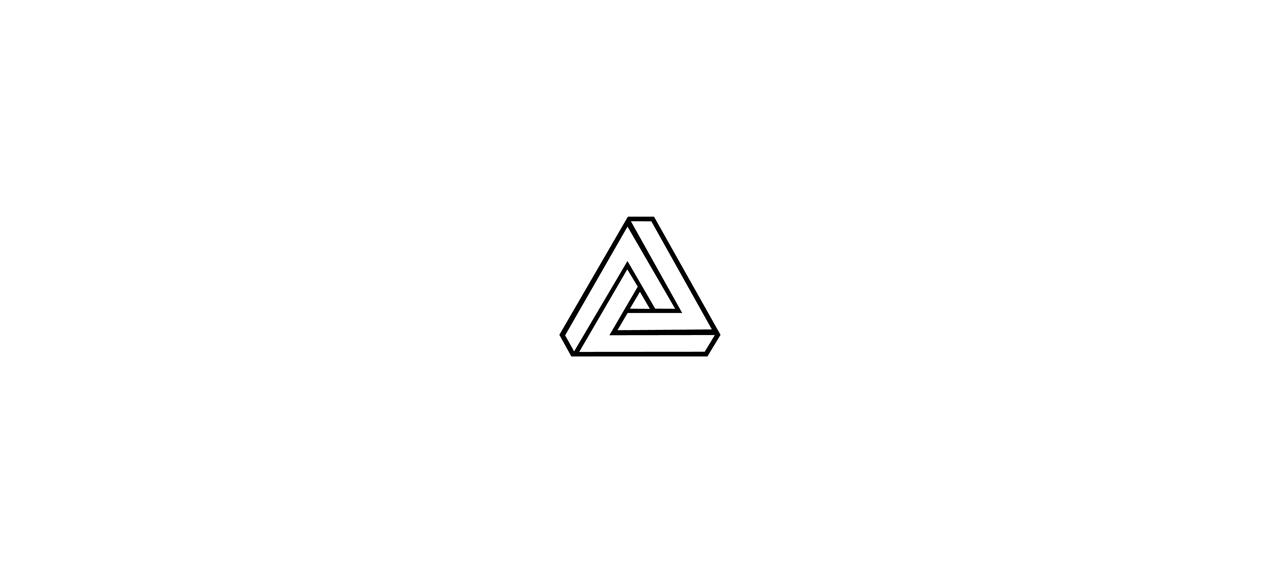
\includegraphics[width=0.8\textwidth]{images/img-001.jpg}\\[2cm]
{\Huge\bfseries Che cos'\`{e} il comunismo?}\\[1cm]
{\large Gruppo Engels}\\[0.5cm]
{\small Traduzione dal russo con \texttt{translategemma:27b}}\\[0.4cm]
{\large 2018}
\vfill
\end{center}
\clearpage

% ── Pagina 3: indice ─────────────────────────────────────────────
\tableofcontents
\newpage
\pagenumbering{arabic}

% ── Sezioni ──────────────────────────────────────────────────────
\subfile{parts/01_inventiamo_occhiali}
\subfile{parts/02_prefazione}
\subfile{parts/03_fondamenti}
\subfile{parts/04_comunismo_realta}
\subfile{parts/05_proprieta_comune}
\subfile{parts/06_opera_necessaria}
\subfile{parts/07_comunismo_gestione}
\subfile{parts/08_comunismo_individuo}
\subfile{parts/09_comunismo_famiglia}
\subfile{parts/10_comunismo_coscienza}
\subfile{parts/11_conclusione}

\end{document}
